% This is a modified version of the tufte-latex book example in which the title page and the contents page resemble Tufte's VDQI book, using Kevin Godby's code from this thread at https://groups.google.com/forum/#!topic/tufte-latex/ujdzrktC1BQ.
%
%% Unfortunately for the contents to contain
%% the "Parts" lines successfully, hyperref
%% needs to be disabled.
\documentclass{tufte-book}
% \usepackage[T2A]{fontenc} % Use 8-bit encoding that has 256 glyphs
\usepackage[OT1]{fontenc} % Use 8-bit encoding that has 256 glyphs
\usepackage[utf8]{inputenc} % Required for including letters with accents
\usepackage[russian]{babel}
% \usepackage{pscyr}
%   \renewcommand{\rmdefault}{ftm}
\usepackage{graphicx}

\title{Конечные структуры \\ {\Huge в примерах}} % The article title

\author{Садыков Нурлан}

% Абстракт
% Заметки по решению кубика рубика с помощью теории групп.

\begin{document}

\frontmatter

\maketitle  
\chapter{Кубик Рубика}
\section{Где здесь группа?}


\begin{marginfigure}
    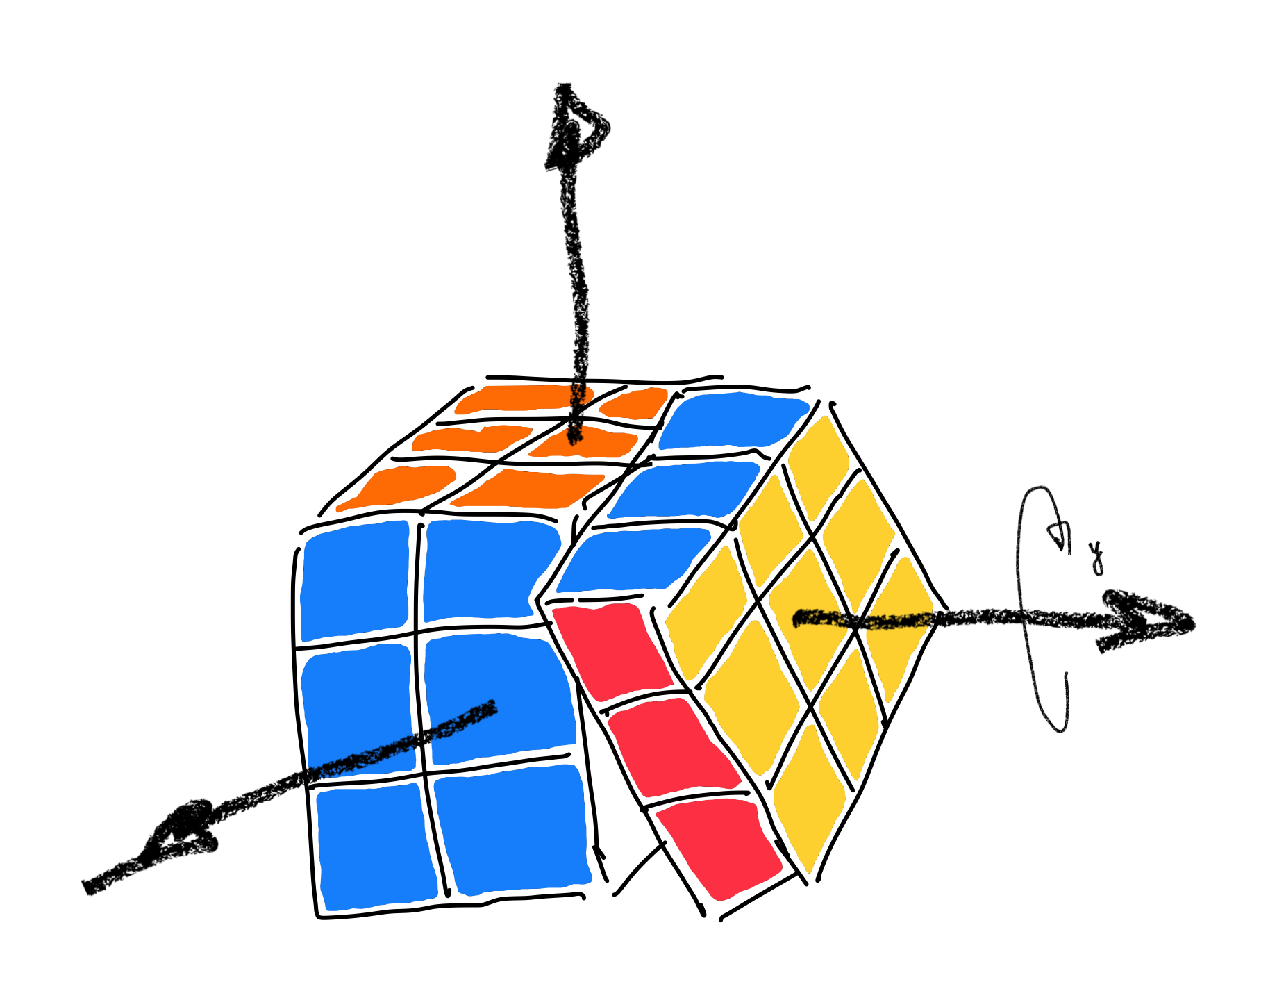
\includegraphics[width=1.1\columnwidth]{../pics/rubik_single_move.pdf}
    \caption{Движение желтой грани $y$}
    \label{fig:move_y}
    %\setfloatalignment{b}
\end{marginfigure}


Обозначим вращения граней кубика\sidenote[][1\baselineskip]{
    Под вращением грани понимаем ее поворот на $90^\circ$ по часовой стрелке
    относительно остальной части кубика.
} в соответствии с
цветом центрального стикера на грани. Это удобно потому, что вращения граней
всегда оставляют центральные стикеры на месте. Будем обозначать эти вращения
цветами соответствующих граней: $o$-оранжевый, $b$-синий, $r$-красный,
$y$-желтый, $w$-белый, $g$-зеленый. Вращения граней кубика рубика являются
образующими свободной группы. Любое слово в этой группе можно применить как
инструкцию к кубику рубика. Будем считать слово тривиальным, если после его
применения к собранному кубику, мы снова получим собранный
кубик.\sidenote[][1\baselineskip]{Любые промежуточные состояния применения слова к кубику не
обязаны давать собранный вариант.} Например, очевидно, что $b^4 = bbbb = e$ то
есть вращение относительно синей грани четыре раза --- тривиальное слово,
поскольку снова дает правильную сборку.

Для определенности будем считать, что мы применяем слова к кубику слева
направо. То есть слово $oby$ это сперва повернуть оранжевую грань на
$90^\circ$, потом синюю и только потом желтую.

\section{Кодировка состояния кубика}
Каждое действие переставляет стикеры на кубике Рубика, значит группа действий
на кубике может быть описана как подгруппа группы перестановок. Чтобы явно
определить перестановку по какому-либо состоянию нужно ввести
кодировку.\sidenote[][1\baselineskip]{\emph{Пример неполной кодировки.} Если цветам приписать
    такие векторы $o=(0,\,0,\,1)$, $b=(1,\,0,\,0)$, $y=(0,\,1,\,0)$,
    $w=(0,\,-1,0)$, $g=(-1,\,0,\,0)$, $r=(0,\,0,\,-1)$, то можно определить
    начальную координату каждого маленького кубика в кубике Рубика как сумму
    цветов входящих в маленький кубик. Так можно было ввести кодировку
    состояния кубика Рубика, но она получится неполной. Чтобы убедиться в этом
    достаточно посмотреть на слово $\alpha = oywgbrowygbr$. Если его применить
    к начальному состоянию, вершинная кодировка покажет тривиальную
    перестановку, но мы не получим начальное состояние. Так происходит потому,
    что это слово меняет ориентацию некоторых кубов на границах двух цветов.
Слово $\alpha^2=e$ уже будет тривиальным.}

Для удобства мы будем обозначать элементы цветом и индексом, например, $b_5$
будет обозначать центральный синий стиркер. Индексы на каждой грани
определяются в соответствии с рисунком~\ref{fig:representation}.

Как только мы ввели кодировку, можем проследить какой стикер стоит на какой позиции. И уже отсюда можем вытащить перестановки.


\begin{marginfigure}
    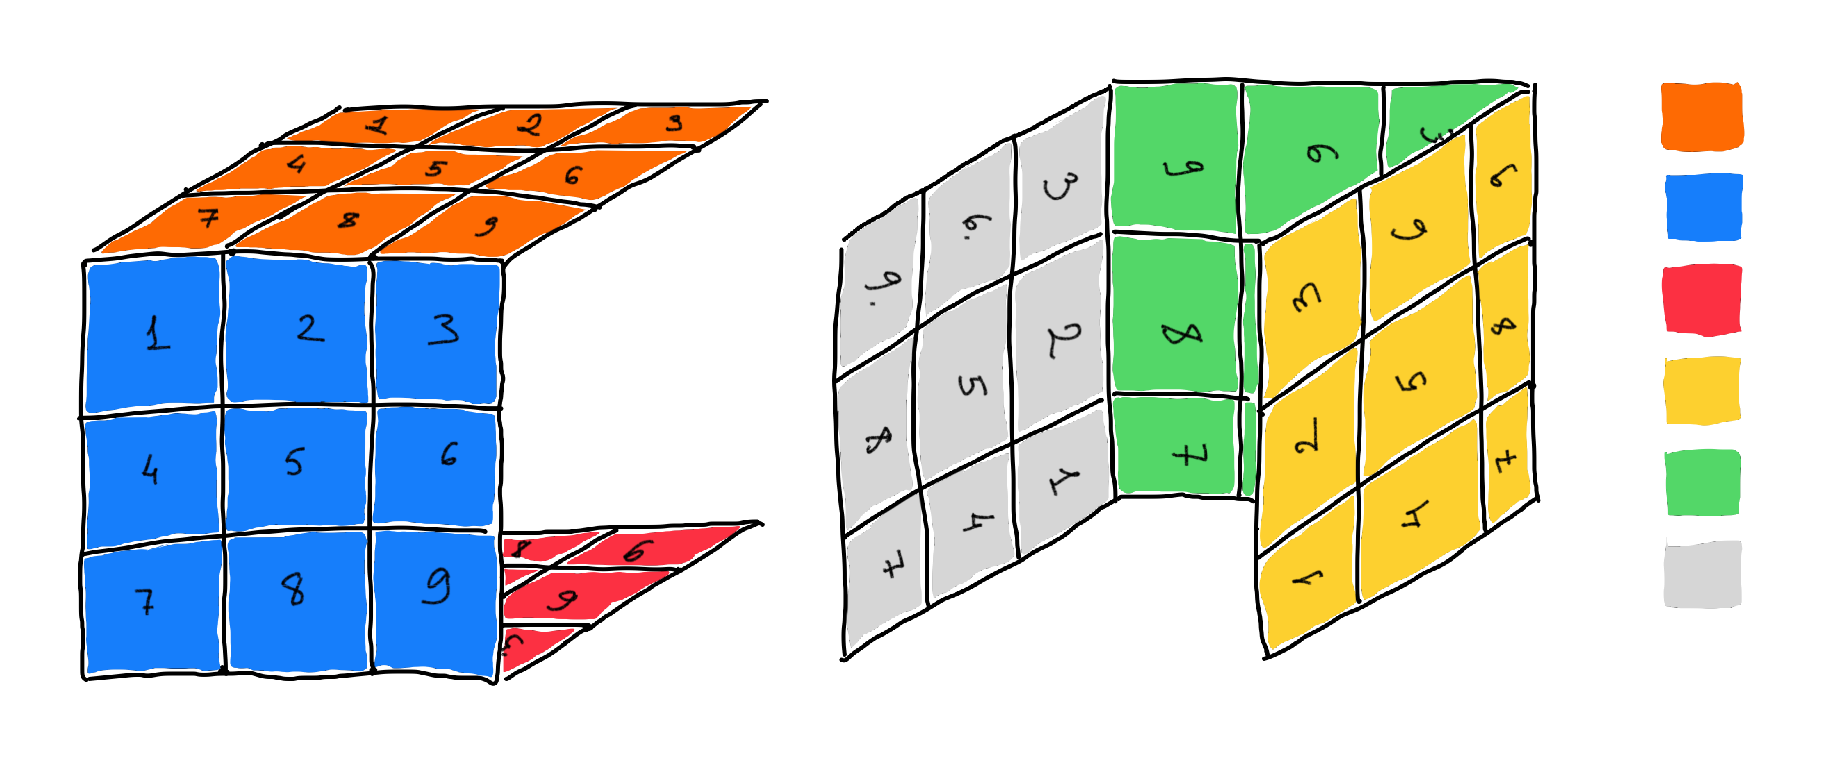
\includegraphics[width=1.1\columnwidth]{../pics/rubik_prepresentation.pdf}
    \caption{Движение желтой грани $y$}
    \label{fig:representation}
    %\setfloatalignment{b}
\end{marginfigure}

\subsection{Как так}

\end{document}
